\chapter{LHC and the CMS experiment}
\chaptermark{The LHC and the CMS experiment}  
\thispagestyle{plain}  % First page has default style
\pagestyle{chapterpages}
\label{Section:Chapter3}

The physics analyses presented in this thesis are performed using data generated by the LHC and collected by the \ac{CMS} experiment. This chapter begins by exploring how the LHC accelerates and collides protons up to centre-of-mass energies ($\sqrt{s}$) of $13.6\TeV$, creating the extreme but necessary conditions needed for rigorous tests of the SM at the electroweak scale. The discussion then shifts to the CMS detector, a multipurpose apparatus composed of several layers of specialised subdetectors. These intricate systems work in concert to enable the precise reconstruction of particles emerging from proton-proton collisions at the heart of the detector.

\section{The LHC}

The LHC~\cite{LHC_1}, situated at the European Organization for Nuclear Research (CERN) near Geneva, Switzerland, is a testament to human scientific achievement. Ingeniously, the LHC was placed within the tunnel previously occupied by the Large Electron Positron (LEP) collider. Engineered to facilitate proton-proton (pp) collisions, the machine was designed to generate such collisions with centre-of-mass energy up to $14\TeV$ and an unprecedented luminosity of $10^{34}\unit{cm}^{-2}\unit{s}^{-1}$. As mentioned earlier, the LHC is currently running just below its maximum energy capabilities, with each beam carrying $6.8\TeV$ of energy. Spanning a circumference of $27\unit{km}$, the LHC mirrors the basic layout of its predecessor, LEP, as illustrated in Fig~\ref{Figure:Chapter3_LHC_BasicLayout}. 

\begin{figure}[h]
\centering
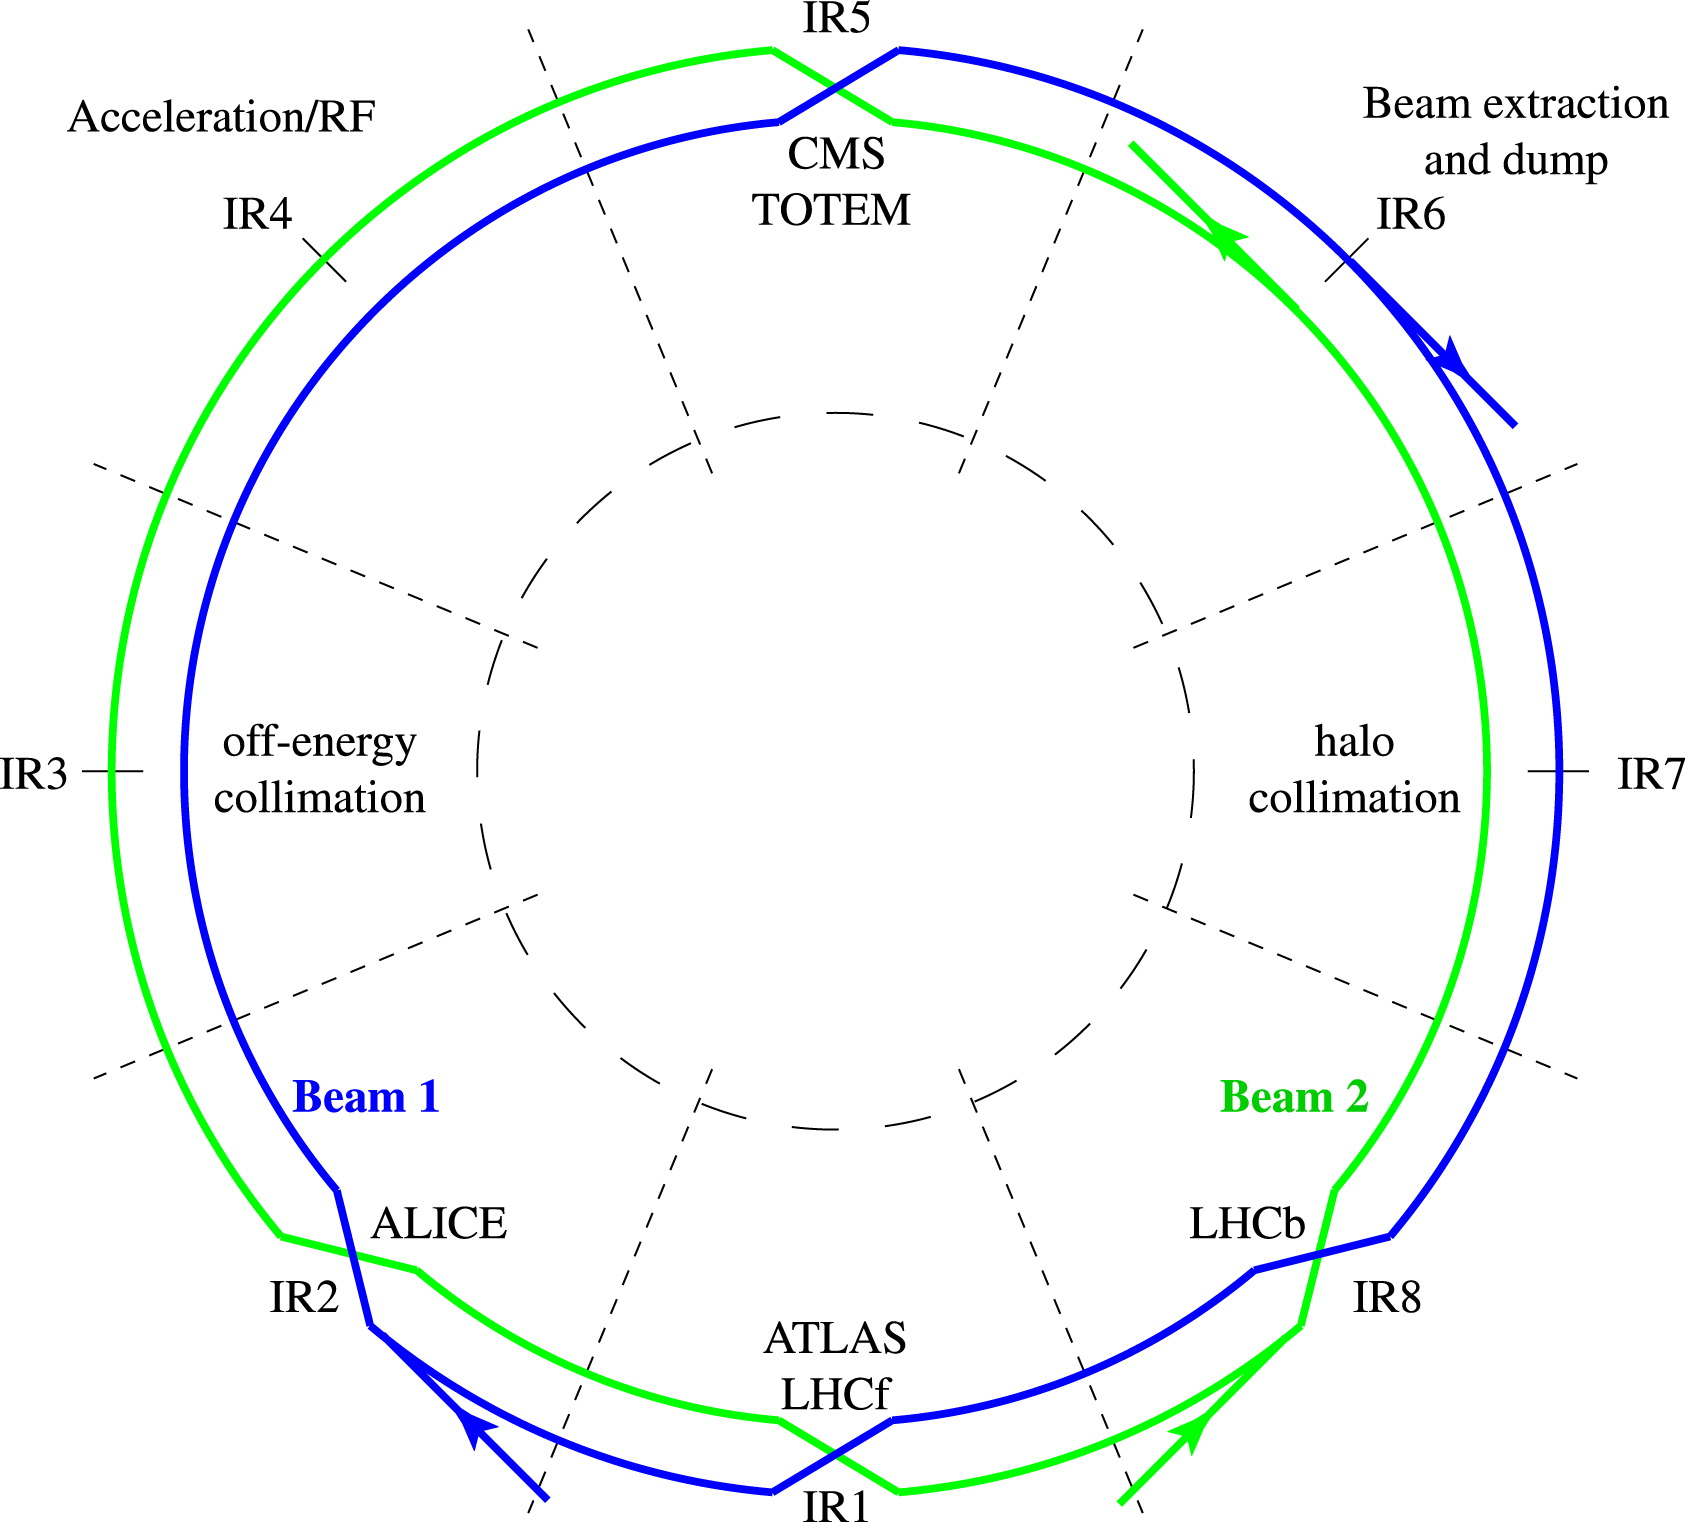
\includegraphics[width= 0.7\textwidth]{Figures/Chapter3/LHC_BasicLayout.jpg}
\caption{Basic schematic layout of the LHC consisting of 8 arc sections along with the two circulating beams and the ATLAS, ALICE, CMS, and LHCb experiments~\cite{LHC_BasicLayout}.}
\label{Figure:Chapter3_LHC_BasicLayout}
\end{figure}

The experimental landscape is strategically arranged with two general-purpose experiments, ATLAS~\cite{LHC_ATLAS} and CMS~\cite{LHC_CMS}, positioned at diametrically opposite sections, at Points 1 and 5 respectively. The ALICE experiment~\cite{LHC_ALICE} occupies Point 2, while LHCb~\cite{LHC_LCHb} is situated at Point 8. At these critical locations, the circulating beams are precisely focused and brought into collision.

Particles are not accelerated to an energy of $6.8~\TeV$ per beam simply by circulating in the LHC tunnel. Instead, the LHC is the final stage of a sophisticated accelerator chain~\cite{LHC_InjectorComplex} at CERN, in which a series of machines successively boost the energy of the particles, as shown in Fig.~\ref{Figure:Chapter3_LHC_Complex}. The first step in this accelerator complex is the Linear Accelerator 4 (LINAC4)~\cite{LINAC4}, which produces a beam of negative hydrogen ions ($\text{H}^-$), each consisting of a proton and two electrons. LINAC4 accelerates these ions to an energy of $160\MeV$ before injecting them into the Proton Synchrotron Booster (PSB). During injection, the electrons are stripped off, leaving behind bare protons. The PSB then accelerates the protons to a kinetic energy of $2.0\GeV$. Next, the beam is transferred to the Proton Synchrotron (PS), which increases its energy to $26\GeV$. From there, the particles are sent to the largest machine in the injector complex, the Super Proton Synchrotron (SPS), which boosts their energy to $450\GeV$. Throughout the injector chain, the protons are grouped into bunches, which are subsequently injected into the two concentric beam pipes of the LHC as two counter-rotating beams. The injection continues until each beam consists of 2808 bunches, separated by $25\unit{ns}$.

\begin{figure}[h]
\centering
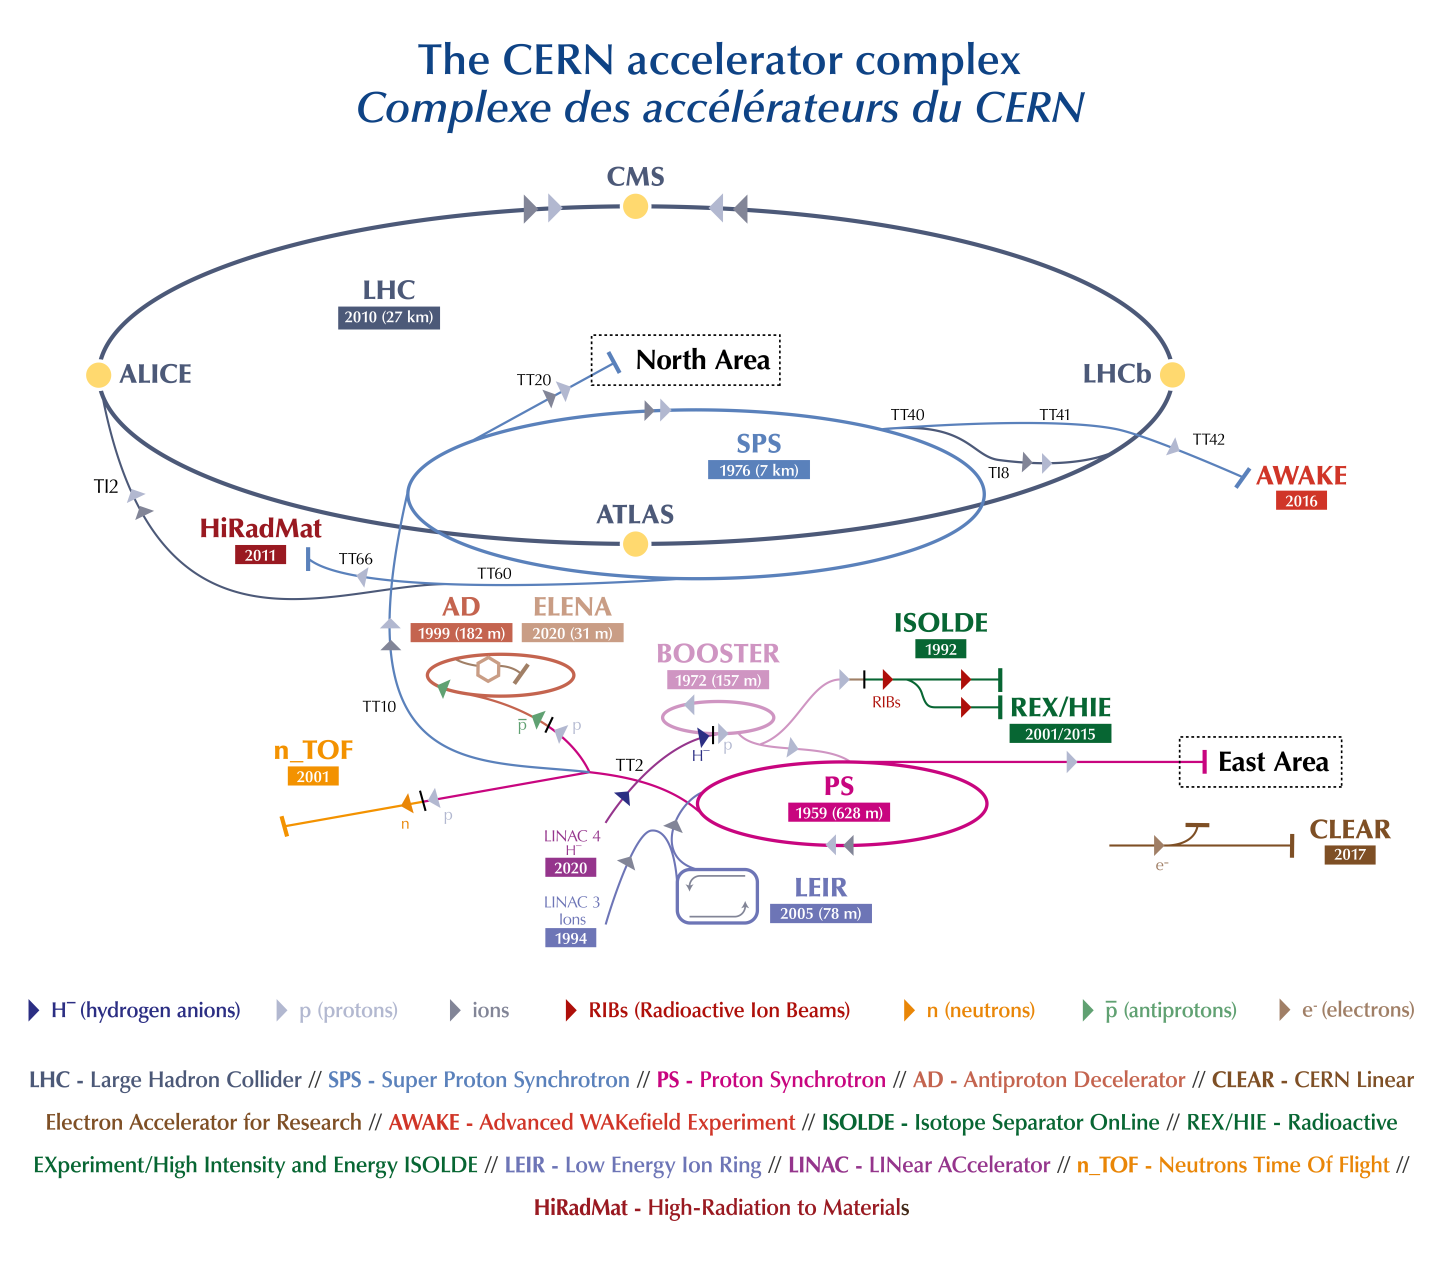
\includegraphics[width= 1.0\textwidth]{Figures/Chapter3/LHC_AcceleratorComplex.png}
\caption{Schematic diagram of the CERN accelerator complex~\cite{LHC_InjectorComplex}.}
\label{Figure:Chapter3_LHC_Complex}
\end{figure}

A network of 1232 superconducting (niobium-titanium) dipole magnets bend the beams along the circular LHC ring. These magnets operate at ultra-low temperatures of $1.9\unit{K}$, achieved using superfluid helium, and can produce magnetic fields up to $8.4\unit{T}$. Beam acceleration is facilitated by sixteen $400\unit{MHz}$ radiofrequency (RF) cavities, providing a \~14-fold energy increase compared to the injection energy. The circular trajectory of the accelerating beams is maintained by dynamically adjusting the magnetic field strength of the dipole magnets, while 392 quadrupoles are utilised to focus the beams. Just before the collision at each of the four principal points, four inner triplet quadrupole magnets are used to reduce the transverse size of the beams. This effectively squeezes them, aiming to maximise the collision rate~\cite{LHC_Run3}, as illustrated in Fig.~\ref{Figure:Chapter3_LHC_BeamSqueeze}. The specifications mentioned above reflect the state of the accelerator complex following the upgrades carried out during the latest scheduled long shutdown, which was completed in 2021.

\begin{figure}[h]
\centering
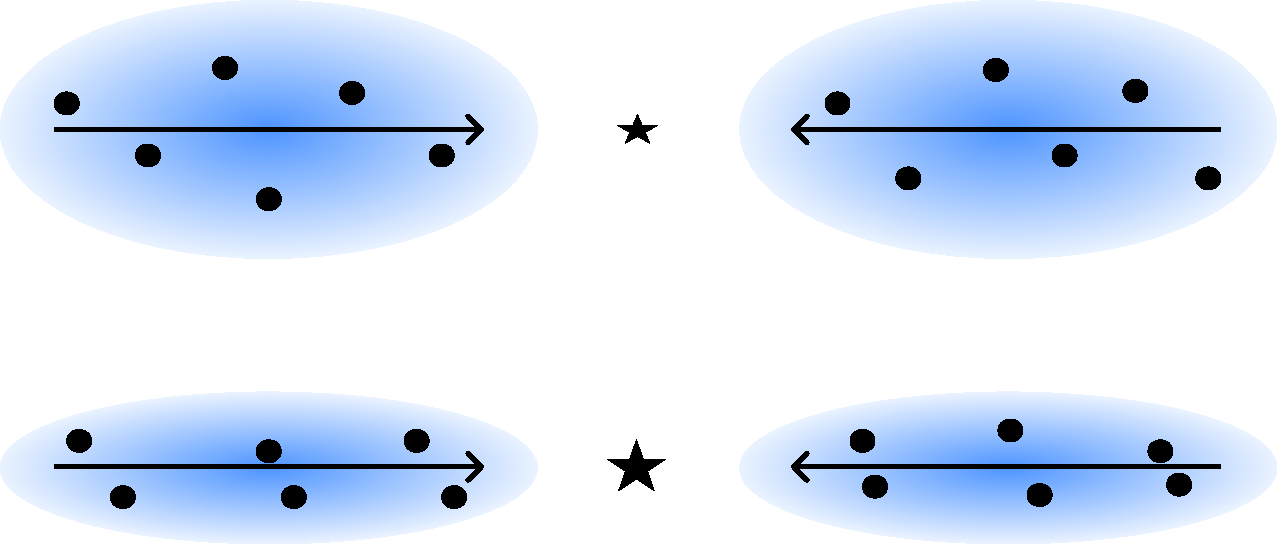
\includegraphics[width= 0.7\textwidth]{Figures/Chapter3/LHC_BeamSqueeze.pdf}
\caption{Illustration of beam squeezing prior to colliding in the heart of detectors at the LHC.}
\label{Figure:Chapter3_LHC_BeamSqueeze}
\end{figure}

\subsection{Cross section and Luminosity}

Cross section and luminosity are essential in understanding and measuring what happens in collider collisions. Together, these determine how often specific physical processes occur in the detector. The cross-section ($\sigma$) describes the probability of a particular process occurring during a collision. Many different processes can occur as the beams cross in the heart of the LHC detectors. The cross-section of each of these processes depends on the type and the energy of the colliding particles, $\sigma(\sqrt{s})$. The cross-section is combined with the instantaneous luminosity ($\mathscr{L}$) to calculate how often a particular process occurs at a collider. Instantaneous luminosity is a measure of how tightly particles are packed into a given space, and it is a function of the beam parameters~\cite{LHC_HL},

\begin{equation}
\begin{aligned}
    \mathscr{L} &= \gamma \frac{n_b N^2 f_{\text{rev}}}{4\pi \beta^* \epsilon_n} R \\
    R &= 1 / \sqrt{1 + \left( \frac{\theta_c \sigma_z}{2\sigma} \right) }
\end{aligned}
\end{equation}

where $\gamma$ is the proton beam energy expressed in rest mass units, $n_b$ is the number of bunches per beam, $N$ is the number of particles per bunch, $f_{rev}$ is the revolution frequency ($11.2\unit{kHz}$), $\beta^*$ is the beam beta function at the collision point and $\epsilon_n$ is the normalised transverse beam emittance. The term R is a geometrical reduction factor for luminosity. This is expressed as a function of the crossing angle of the beams at the collision point ($\theta_c$) and the transverse (longitudinal) spread of the particle bunch, $\sigma_z(\sigma)$. 

The cross-section, together with the instantaneous luminosity, determines the rate (R) at which a given process occurs in the detector,

\begin{equation}
    R = \sigma(\sqrt{s}) \cdot \mathscr{L} 
\end{equation}

The beam parameters are constant over time; hence, the luminosity varies. A more appropriate quantity is the integrated luminosity ($\mathscr{L}_{int}$), which considers the total data collected over a given period,

\begin{equation}
    \mathscr{L}_{int} = \int \mathscr{L}(t) dt
\end{equation}

In a given period, the total number of events (N) for a particular process with cross-section $\sigma$ can be expressed as:

\begin{equation}
    \mathscr{N} = \sigma \cdot \mathscr{L}_{int}
\end{equation}

A summary of the total integrated luminosity delivered to the CMS experiment since 2015 is provided in Fig.~\ref{Figure:Chapter3_CMS_IntegratedLumi}.

\begin{figure}[h]
\centering
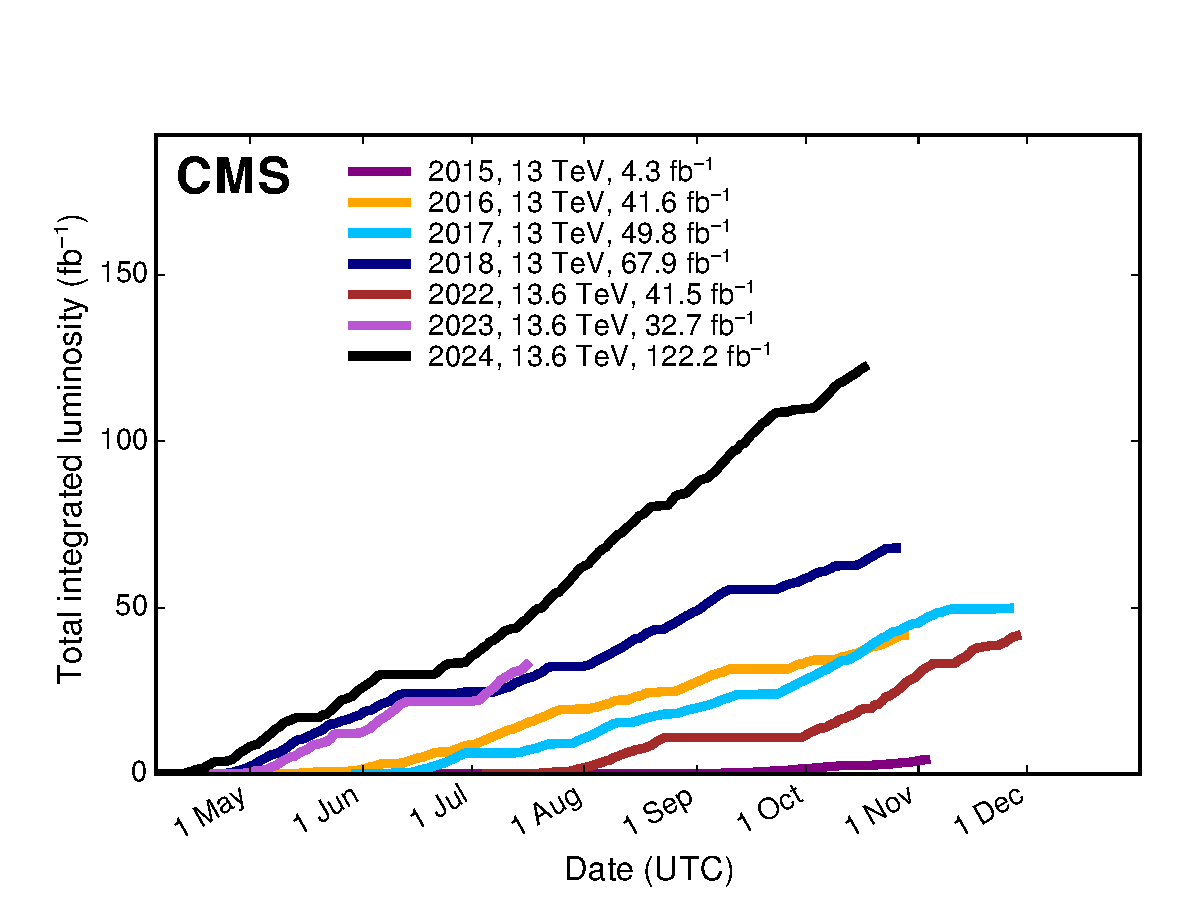
\includegraphics[width= 0.7\textwidth]{Figures/Chapter3/CMS_IntegratedLumi.pdf}
\caption{Total integrated luminosity delivered to the CMS experiment between 2015 to 2024. Data collected from all periods except 2015 and 2024 are used in this thesis. Figure is taken from Ref.~\cite{CMS_IntegratedLumi}.}
\label{Figure:Chapter3_CMS_IntegratedLumi}
\end{figure}

\subsection{Pileup}

The CMS experiment set out to investigate the rarest interactions of proton collisions. In the effort of maximising the chances of observing such rare events, the LHC collides large bunches of protons rather than single protons, as discussed earlier. This approach increases the instantaneous luminosity, which is favourable because it directly enhances the probability of rare processes occurring within a given time. However, this also introduces challenges: when bunches collide, multiple protons interact simultaneously. In other words, CMS records particles from the interaction of interest and particles originating from multiple additional interactions, called pileup interactions. Increasing the instantaneous luminosity leads to the enhancement of pileup. The removal of these unwanted overlap collisions requires increasingly more sophisticated techniques. Figure~\ref{Figure:Chapter3_CMS_Pileup} illustrates the pileup conditions encountered by the CMS experiment between 2015 and 2024.

\begin{figure}[h]
\centering
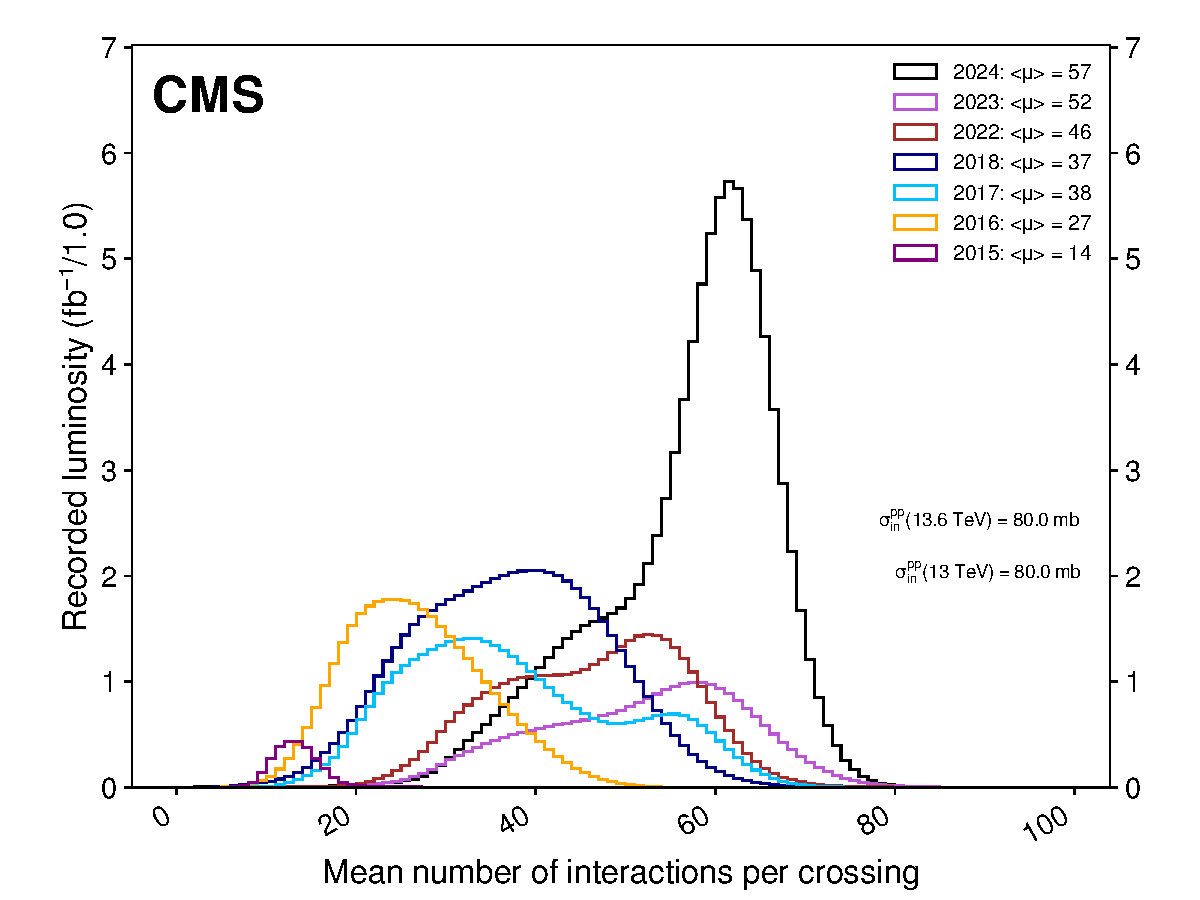
\includegraphics[width= 0.7\textwidth]{Figures/Chapter3/CMS_Pileup.pdf}
\caption{Distribution of average number of interactions per crossing for pp collisions between 2015 to 2024 using data from the CMS experiment, taken from Ref.~\cite{CMS_IntegratedLumi}.}
\label{Figure:Chapter3_CMS_Pileup}
\end{figure}

\section{The CMS Detector}

As previously discussed, CMS is one of the two general-purpose detectors at the LHC, built to explore a wide range of high-energy physics phenomena. The design of the CMS detector was shaped by the ambitious goals of the LHC physics programme, which demanded precise and efficient measurements under challenging experimental conditions. To accomplish these objectives, several key performance requirements were identified:

\begin{itemize}
    \item Identification and precise momentum reconstruction of muons over a broad range of momenta and angles. A dimuon mass resolution of approximately 1\% at 100$\GeV$ is required, along with the ability to determine the charge of muons with momenta below 1$\TeV$ unambiguously.

    \item Good momentum resolution and reconstruction efficiency for charged particles in the inner tracking system. Efficient identification of $\tau$ leptons and b-jets, necessitating fine granularity tracking close; required to locate signatures consistent with secondary interaction vertices.

    \item Electromagnetic energy measurements with excellent resolution for photons and electrons. Diphoton and dimuon mass resolutions of approximately 1\% at 100$\GeV$ is required over a wide geometrical coverage.

    \item Effective $\pi^0$ rejection to distinguish isolated photons from those originating in neutral pion decays. Additionally, efficient isolation of photons and leptons is required, particularly in high-luminosity environments with significant detector occupancy.

    \item Good dijet mass and \ac{MET} resolution are required, necessitating fine laterally segmented hadronic calorimeters providing a near-complete hermetic coverage.
\end{itemize}

CMS employs a compact, layered detector system arranged cylindrically around the interaction point to fulfil these performance requirements, providing a near-complete solid-angle coverage. The entire detector is $21.6\unit{m}$ long and has a diameter of $14.6\unit{m}$ while weighing $12500\unit{t}$. This makes CMS one of the most massive yet \textbf{compact} detectors ever engineered for a particle physics experiment. Closest to the beam pipe lies the silicon tracker, which precisely tracks charged particles. It is surrounded by the Electromagnetic Calorimeter (ECAL), optimised for measuring the energy of electrons and photons with high precision. The Hadronic Calorimeter (HCAL) follows and is responsible for absorbing and measuring the energy of hadrons. These three subsystems are enclosed within a powerful $13\unit{m}$ long, $6\unit{m}$ inner-diameter, $3.8\unit{T}$ superconducting \textbf{solenoid}. The solenoid. This strong field bends the trajectories of charged particles, enabling precise momentum measurements. Embedded within the iron return yoke of the solenoid is the \textbf{muon} detection system. A schematic of the detector layout is shown in Fig.~\ref{Figure:Chapter3_CMS_schematic}. Each of the main detector subsystems introduced here will be discussed in more detail in the following sections of this chapter.


\begin{figure}[h]
\centering
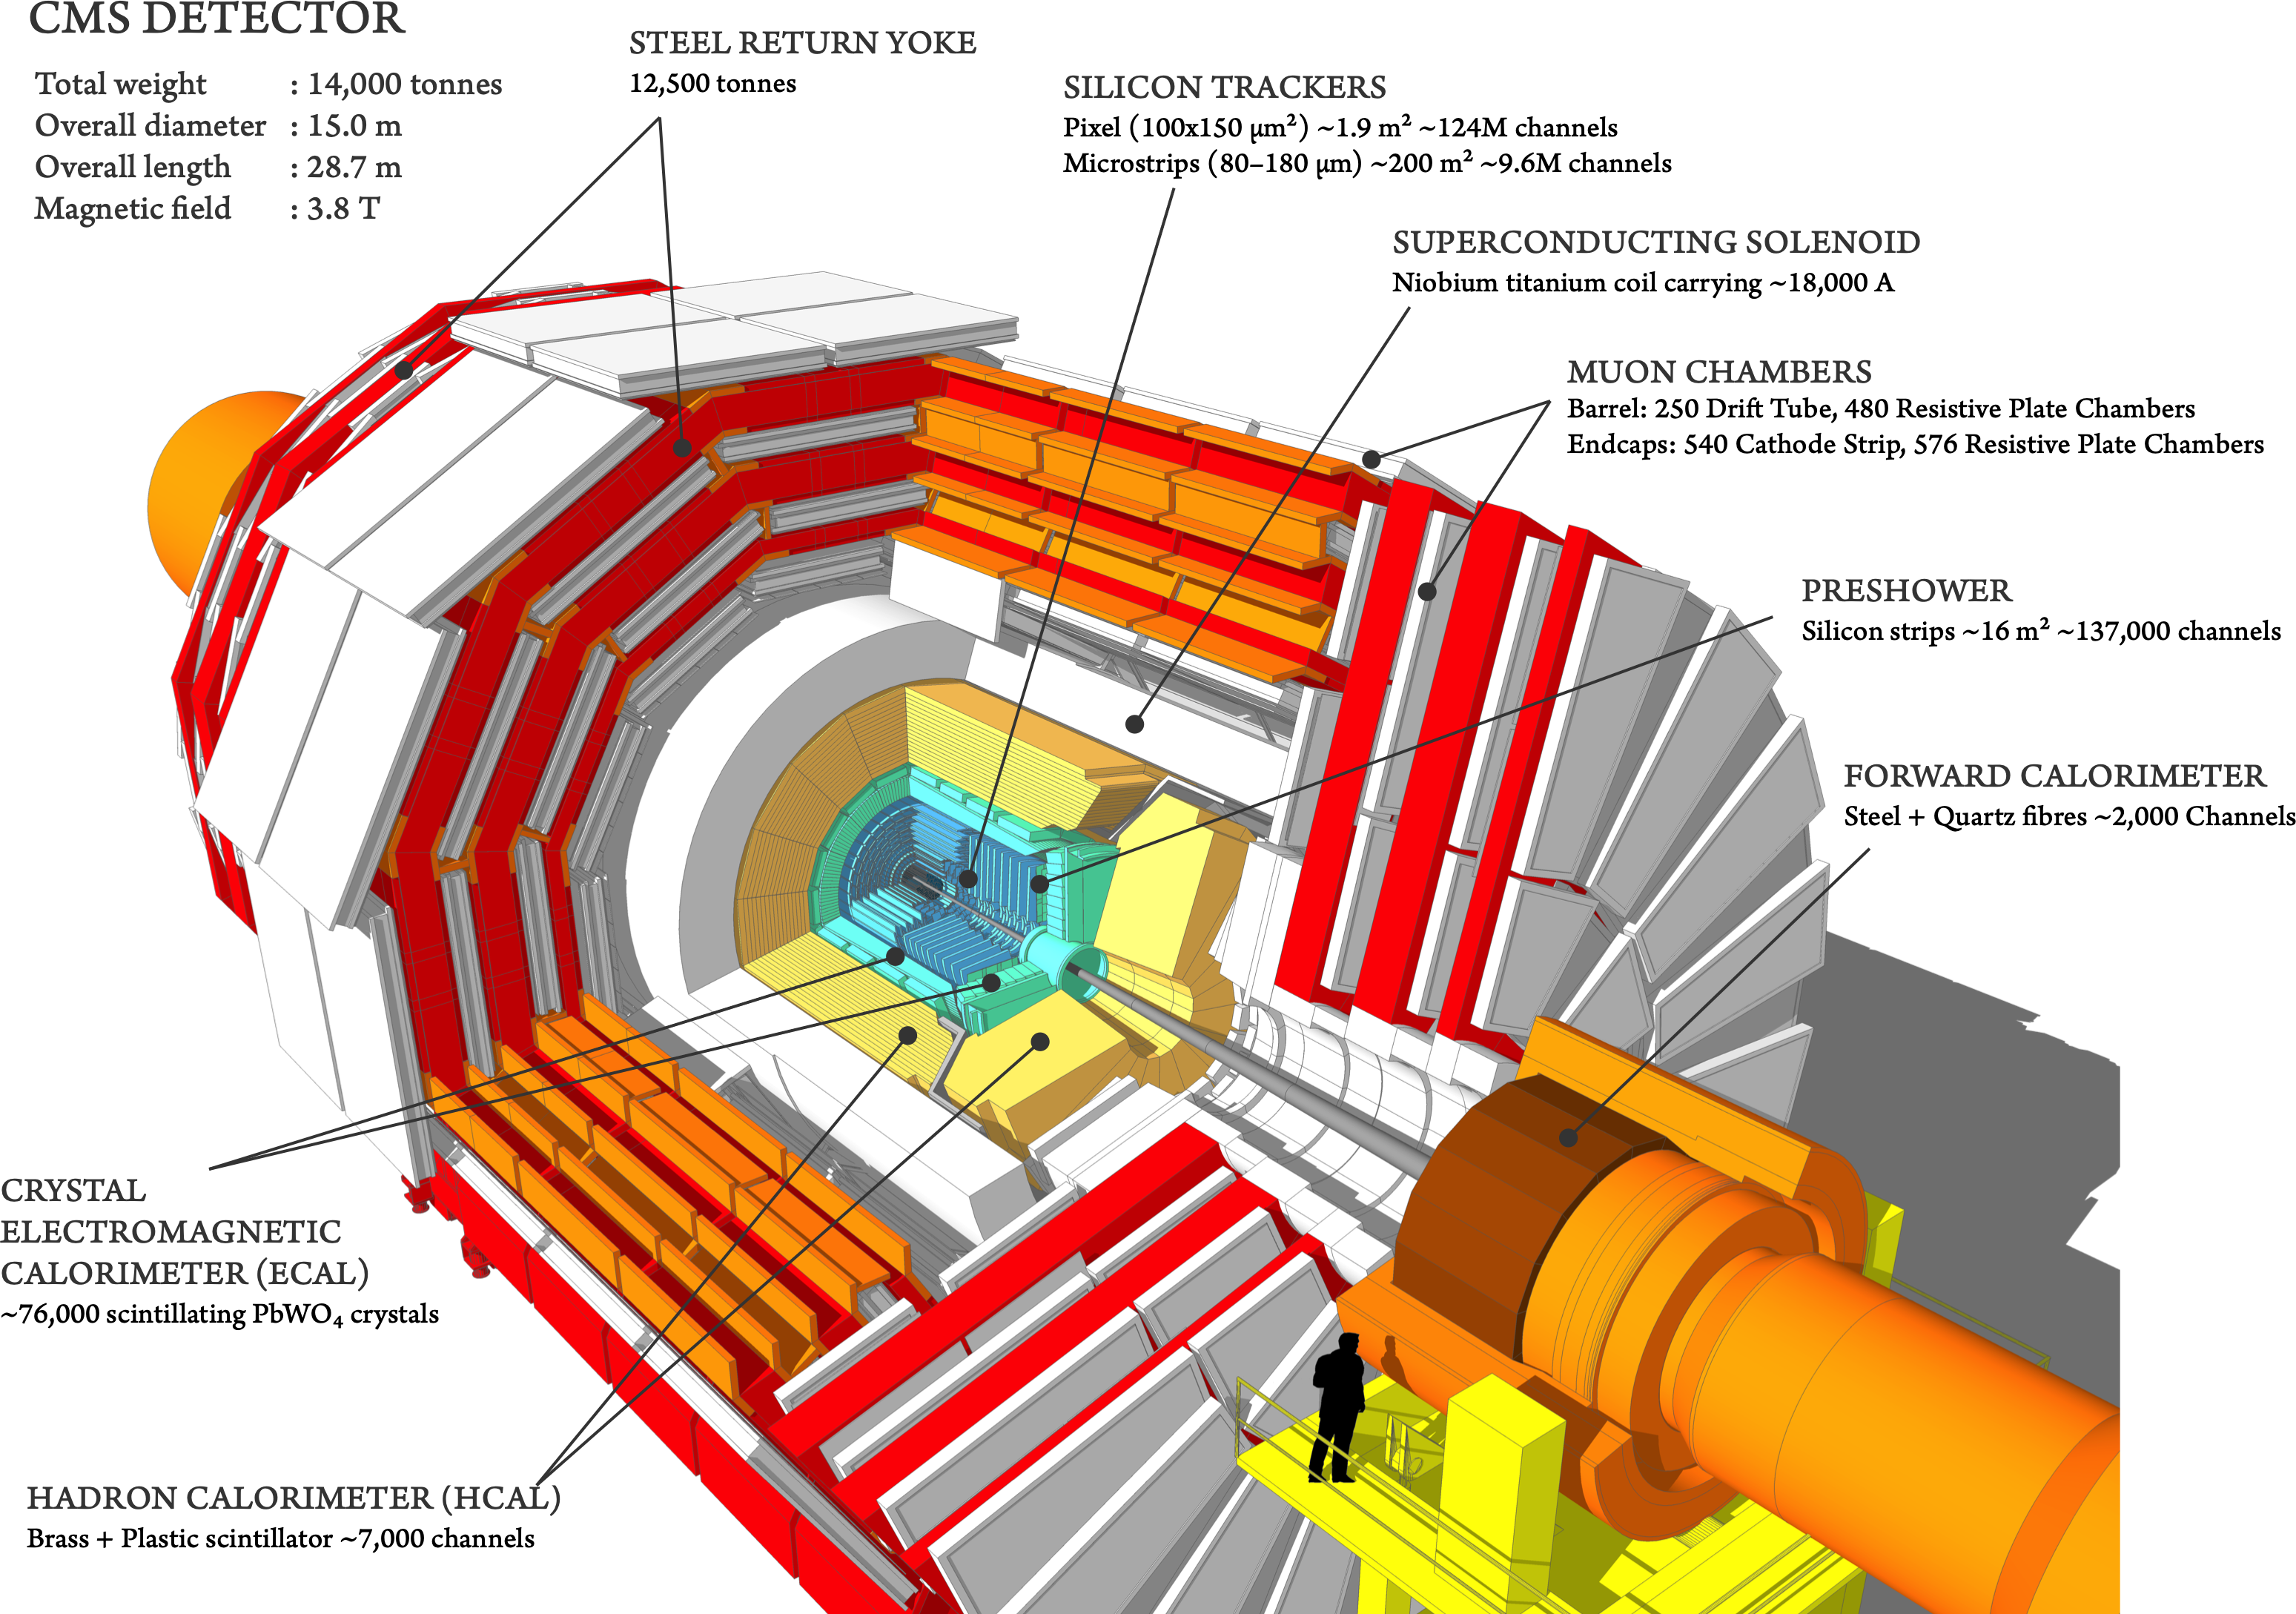
\includegraphics[width= 1\textwidth]{Figures/Chapter3/CMS_Detector.png}
\caption{Schematic drawing of the CMS detector, taken from Ref.~\cite{CMS_Detector_Run3}.}
\label{Figure:Chapter3_CMS_schematic}
\end{figure}


\section{}